\subsection{2026-09-21 --- Exploratory data analysis}
\label{sec:eda}

Full notebook: \texttt{src/EDA/eda.ipynb}. Figures below are extracted from its executed
outputs; see \texttt{figures.md} for exact provenance per figure.

\subsubsection*{Target: per-unit imbalance and correlation structure.}

\begin{figure}[htbp]
  \centering
  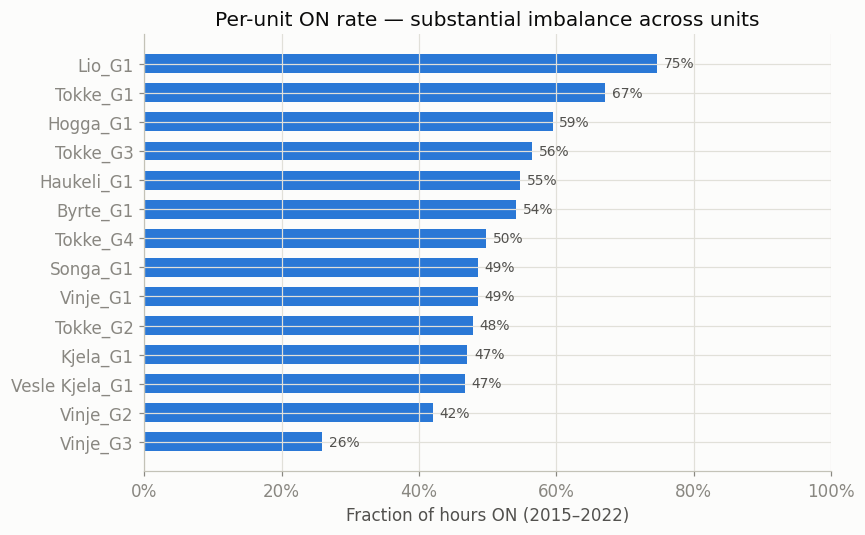
\includegraphics[width=0.75\linewidth]{figures/eda_01_unit_on_rate.png}
  \caption{Per-unit ON rate, 2015--2022.}
  \label{fig:eda-unit-on-rate}
\end{figure}

\finding{ON rate varies from 26\% (Vinje\_G3) to 75\% (Lio\_G1) across units
(Figure~\ref{fig:eda-unit-on-rate}) --- this is not one balanced binary problem, and per-unit
performance should be tracked separately, not just the pooled micro-AUC.}

\begin{figure}[htbp]
  \centering
  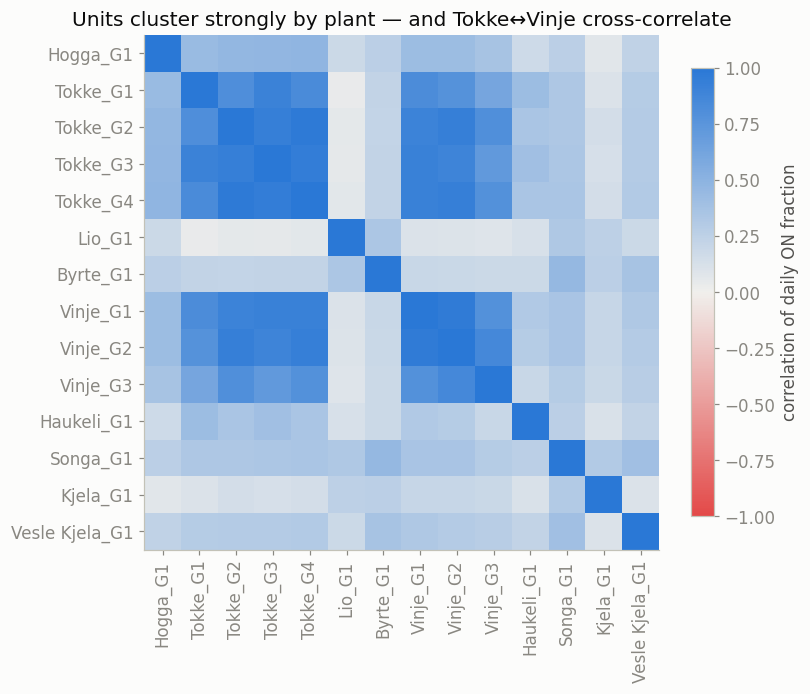
\includegraphics[width=0.75\linewidth]{figures/eda_02_unit_correlation_heatmap.png}
  \caption{Correlation of units' daily ON fraction, ordered by plant.}
  \label{fig:eda-unit-corr}
\end{figure}

\finding{Units at the same plant correlate strongly (0.8--0.96). More notably, Tokke and Vinje
--- different plants, different immediate reservoirs --- also cross-correlate at 0.8--0.9
(Figure~\ref{fig:eda-unit-corr}). This turned out to be explainable by the watercourse
topology: Vinje's reservoir (Vaamarvatn) cascades downstream into Vinjevatn, which is exactly
the reservoir Tokke draws from. This motivates modeling units jointly rather than as 14
independent problems.}

\subsubsection*{Seasonality.}

\begin{figure}[htbp]
  \centering
  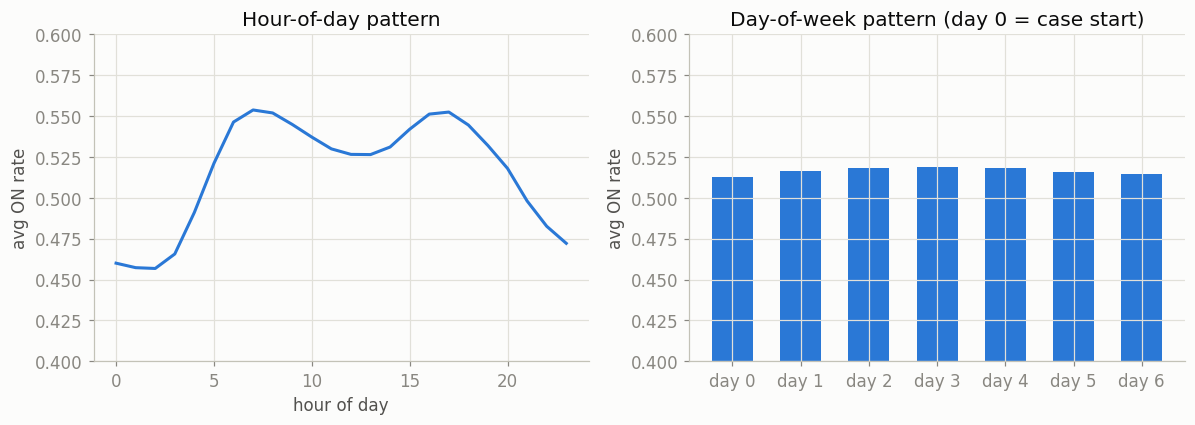
\includegraphics[width=0.95\linewidth]{figures/eda_03_hour_and_dow_pattern.png}
  \caption{ON rate by hour-of-day and by day-of-week within a case.}
  \label{fig:eda-hod-dow}
\end{figure}

\finding{Strong intraday seasonality (double-hump pattern, trough $\approx$0.46 at night,
peaks $\approx$0.55 at the morning/evening demand ramps) but weak day-of-week seasonality
(0.51--0.52 across all 7 days) --- see Figure~\ref{fig:eda-hod-dow}. \texttt{hour\_of\_day} is a
much more informative time feature than \texttt{day\_of\_week} here.}

\subsubsection*{Yearly trend and the 2022 outlier.}

\begin{figure}[htbp]
  \centering
  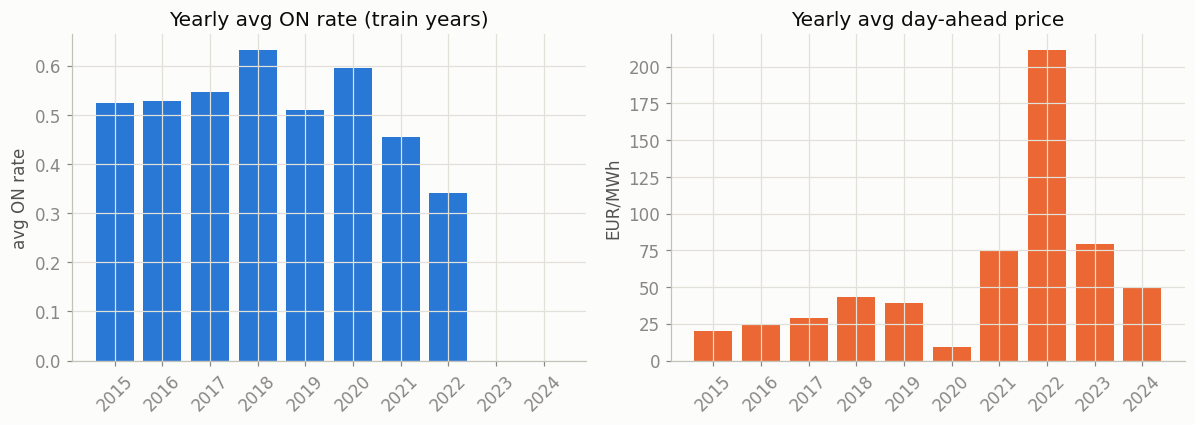
\includegraphics[width=0.75\linewidth]{figures/eda_04_yearly_on_rate_vs_price.png}
  \caption{Yearly average ON rate vs.\ yearly average day-ahead price.}
  \label{fig:eda-yearly}
\end{figure}

\begin{figure}[htbp]
  \centering
  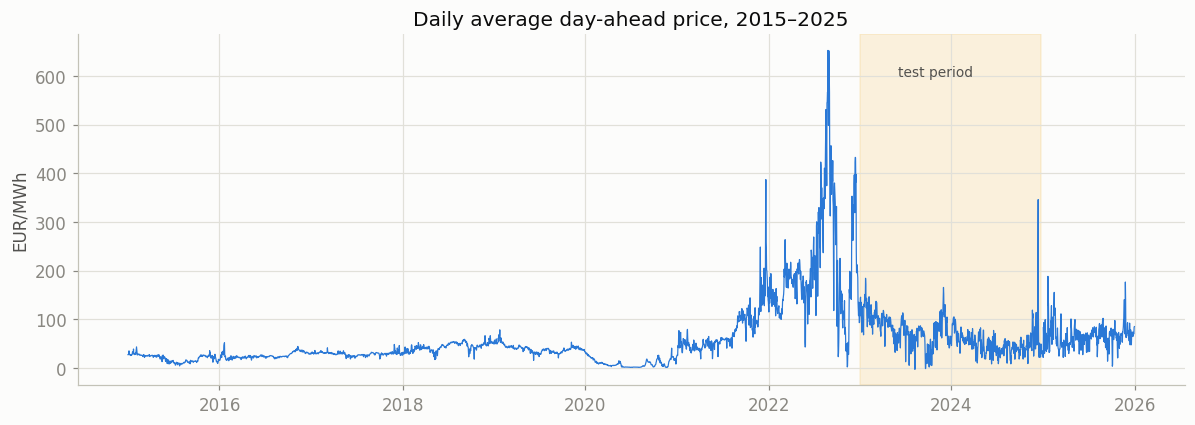
\includegraphics[width=0.85\linewidth]{figures/eda_05_price_timeseries.png}
  \caption{Daily average price, 2015--2025, with the 2023--2024 test window shaded.}
  \label{fig:eda-price-ts}
\end{figure}

\finding{2022 (European energy crisis) has the \emph{highest} average price in the series
($\sim$211 EUR/MWh) but the \emph{lowest} average ON rate (0.34) --- see
Figure~\ref{fig:eda-yearly}. The naive ``high price $\Rightarrow$ more generation'' intuition
does not hold at the year level (explained further below). The 2022 spike sits entirely in the
training window; the test window (2023--2024, shaded in Figure~\ref{fig:eda-price-ts}) is
elevated relative to 2015--2020 but nowhere near the 2022 extreme --- a distribution-shift risk
that motivated a chronological (not random) validation split for modeling.}

\subsubsection*{Physical drivers: inflow, storage, water value.}

\begin{figure}[htbp]
  \centering
  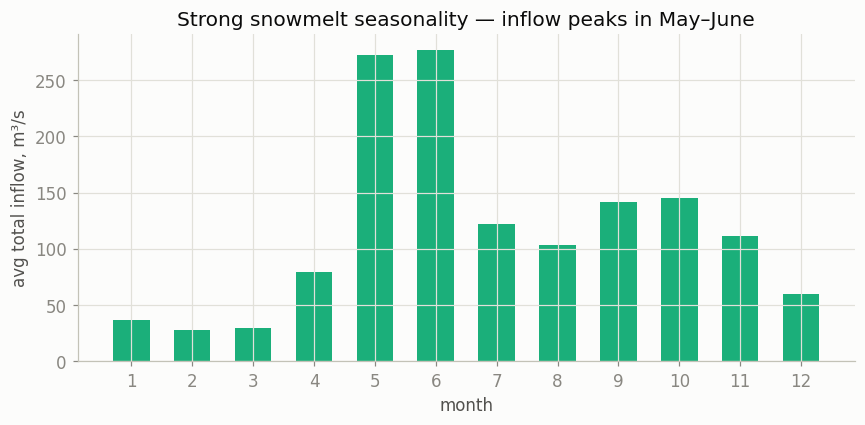
\includegraphics[width=0.7\linewidth]{figures/eda_06_inflow_seasonality.png}
  \caption{Average total reservoir inflow by calendar month.}
  \label{fig:eda-inflow-season}
\end{figure}

\begin{figure}[htbp]
  \centering
  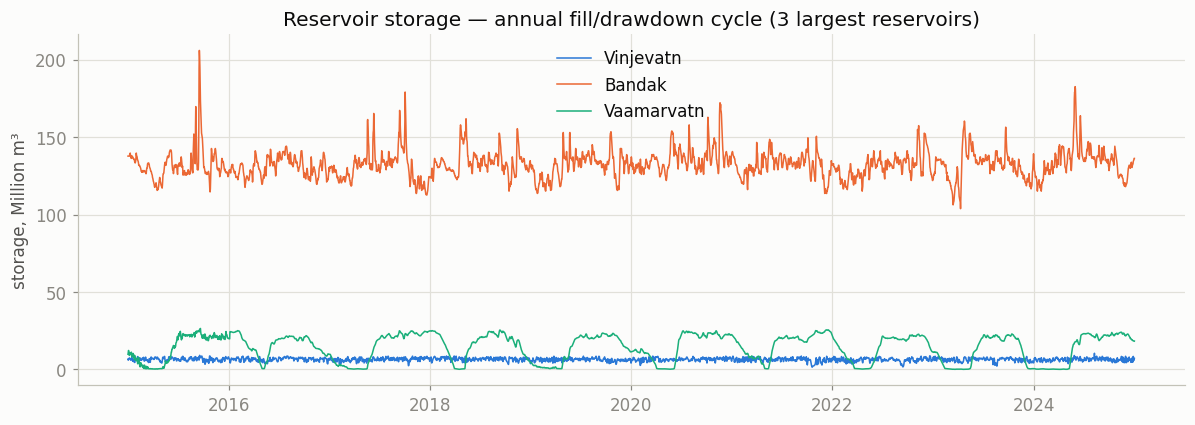
\includegraphics[width=0.85\linewidth]{figures/eda_07_reservoir_storage_cycle.png}
  \caption{Daily storage, three largest reservoirs.}
  \label{fig:eda-storage}
\end{figure}

\begin{figure}[htbp]
  \centering
  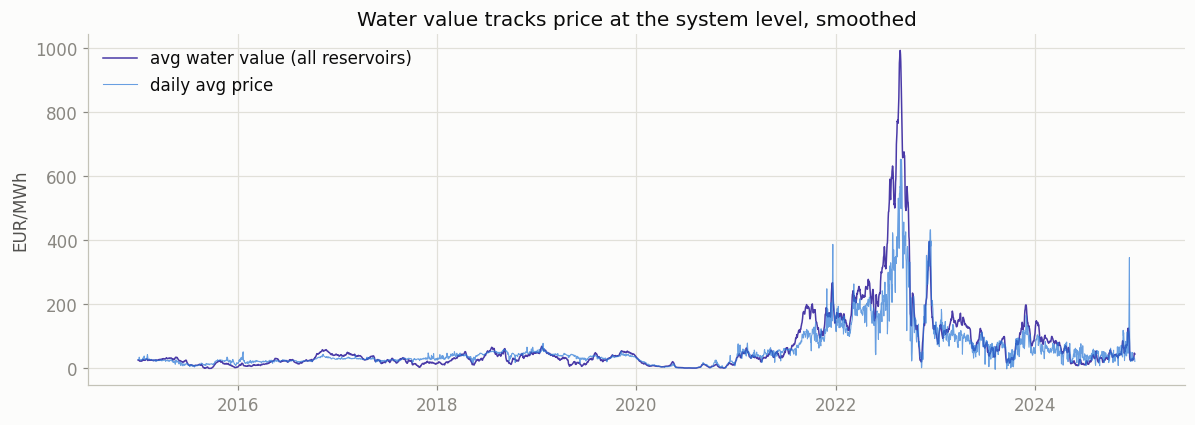
\includegraphics[width=0.85\linewidth]{figures/eda_08_water_value_vs_price.png}
  \caption{System-average water value vs.\ daily average price.}
  \label{fig:eda-wv-price}
\end{figure}

\finding{Classic Norwegian snowmelt seasonality: total inflow across all 17 reservoirs is
$\sim$8$\times$ higher in May--June than in the Jan--Feb trough
(Figure~\ref{fig:eda-inflow-season}), driving the annual storage fill/drawdown cycle
(Figure~\ref{fig:eda-storage}). System-average water value tracks price but is much smoother
(Figure~\ref{fig:eda-wv-price}) --- it reflects the expected \emph{future} value of stored
water, not the instantaneous spot price.}

\subsubsection*{The headline finding: relative price, not absolute price.}

\begin{figure}[htbp]
  \centering
  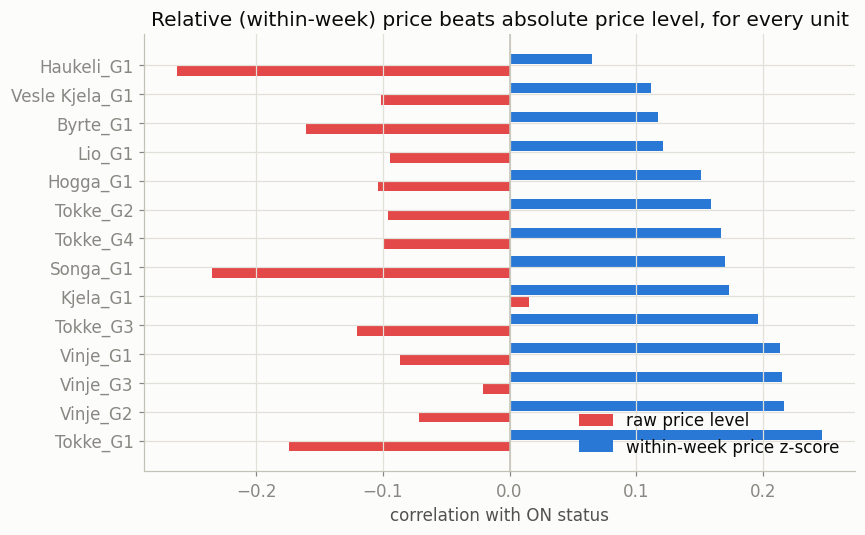
\includegraphics[width=0.75\linewidth]{figures/eda_09_price_corr_raw_vs_within_week_z.png}
  \caption{Per-unit correlation of ON status with raw price vs.\ within-case price z-score.}
  \label{fig:eda-price-corr}
\end{figure}

\finding{For every single unit, correlation with ON status flips from weak/negative
(raw price level) to consistently positive ($\sim$0.15--0.25) when price is normalized
\emph{within each case's own 168-hour window} (Figure~\ref{fig:eda-price-corr}). The optimizer
reacts to ``is this hour relatively good within this week's water/price outlook,'' not to
absolute price. High-price years like 2022 also tend to be scarce-water years, where the
optimizer conserves water and runs fewer units despite high prices --- explaining the
year-level negative relationship in Figure~\ref{fig:eda-yearly}. Implication: within-case
normalized price and a \texttt{price $-$ water\_value} spread are promising engineered features,
likely more robust to the 2022-style regime shift than raw levels.}

\subsubsection*{Extended data.} The topology YAML gives an explicit plant $\to$ upstream-reservoir
map (used above to explain the Tokke/Vinje correlation) and defines the wider reservoir/river/
tunnel graph. The environmental constraint files are sparse and seasonal --- only a handful of
reservoirs/rivers are ever constrained, and only part of the year --- suggesting a binary
``currently constrained'' flag would be a more useful encoding than the raw (mostly-zero)
values, if we decide to use the extended data at all.
